\smalltitle{سوال 3}
\begin{enumerate}
    \item به صورت خیلی خلاصه این روش به ما
    کمک می‌کند که بتوانیم
    \lr{hazard detection}
    را در پردازنده و
    \lr{instruction set}های
    شلوغ و پیچیده، ساده‌تر پیاده سازی کنیم.
    به صورت خیلی خلاصه برای هر رجیستر یک عدد نگه می‌داریم که که چه زمانی دیتایی که می‌خواهیم که در رجیستر بنویسیم مقدارش آماده می‌شود. به عنوان مثال ممکن است که در مرحله بعد از خواندن از رجیستر فایل (یعنی در
    \lr{execute stage})
    مقدار آماده شود. ولی ممکن هم هست که در حالتی در دو مرحله بعد اصلا آماده شود. به
    عنوان مثال زمانی که می‌خواهیم از مموری بخوانیم.
    این عدد هر بار که دستوری را 
    \lr{decode}
    می‌کنیم برای رجیستر مقصد آن مشخص می‌شود.
    دقت کنید که این عدد برای هر دستور متفاوت است (دستوری مثل
    \lr{and}
    در زمان
    \lr{execute}
    داده‌اش آماده می‌شود ولی دستوری مثل
    \lr{load word}
    در
    \lr{MIPS}
    در مرحله‌ی
    \lr{memory}
    آماده می‌شود.)
    
    همچنین زمانی که دستوری را
    \lr{decode}
    می‌کنیم باید چک کنیم که
    \lr{source register}های
    آن، دیتای آنها آماده است یا خیر. برای هر دستور نیز عددی را هاردکد می‌کنیم که نشان می‌دهد که دیتای آن در چند مرحله بعد نیاز می‌شود. مثلا دستور
    \lr{save word}
    در دو مرحله بعد دیتایی که قرار است در
    \lr{memory}
    نوشته شود نیاز می‌شود.
    
    زمانی که دستوری را
    \lr{decode}
    می‌کنیم در ابتدا به
    \lr{source register}های
    آن و اعدادی که به آنها نسبت داده‌ایم نگاه می‌کنیم. در صورت نیاز
    \lr{forwarding}، \lr{stall} یا هیچ کاری
    انجام نمی‌دهیم.
    \item در این روش برای هر رجیستر یک عدد نگه می‌داریم که نشان می‌دهد که دیتای
    آن در چند مرحله بعد آماده می‌شود. این عدد حداکثر به اندازه‌ی
    \lr{stage}های
    \lr{pipeline}
    است و به عنوان مثال در معماری
    \lr{powerpc}
    که در مقاله نیز آماده بود این عدد بین ۰ تا ۲ است.
    کاری که باید با این عدد انجام دهیم صرفا یکی مقایسه است و دیگر کم کردن یک از آن. در این حالت صرفا به دو بیت برای نگه داری هر عدد نیازمندیم.
    
    به صورت کلی این روش نیاز ما به
    \lr{hardwire}
    کردن را کمتر می‌کند و اجازه می‌دهد که صرفا با تعریف کردن درست
    \lr{instruction}ها
    بتوانیم به راحتی و سیم بندی کم و به صورت کاملا
    \lr{dynamic}،
    \lr{hazard}
    را تشخیص دهیم.
    
    \item زمانی که یک دستور
    \lr{decode}
    می‌شود، با توجه به مقدار
    $T_{\text{new}}$
    و
    $T_{\text{use}}$
    و مراجعه به جدول زیر می‌توان تشخیص داد که در حال حاضر باید چی کار کرد.
    \begin{figure}[H]
        \centering
        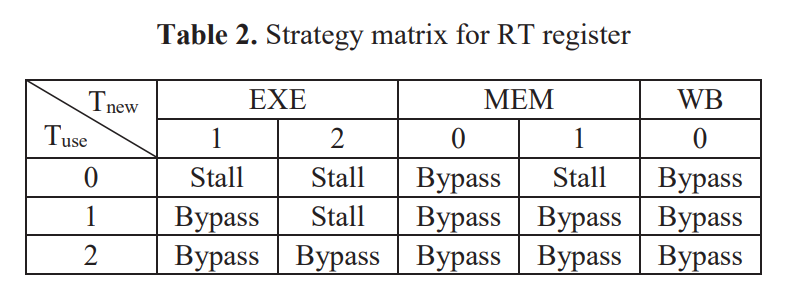
\includegraphics[scale=0.5]{pics/StrategyMatrix.png}
    \end{figure}
    به صورت خیلی خلاصه این جدول به ما می‌گوید که اگر
    $T_{\text{use}} \ge T_{\text{new}}$
    بود، یعنی اینکه دیتا آماده شده است و می‌تواند
    \lr{forward} یا \lr{bypass}
    انجام گیرد. اما از طرفی در صورتی که
    $T_{\text{use}} < T_{\text{new}}$
    بود نشان می‌دهد که دیتای بعدی هنوز آماده نیست و نیاز داریم که صبر کنیم. پس پایپلاین را نگه می‌داریم.
\end{enumerate}